\documentclass[11pt]{article}
\usepackage[margin=0.85in]{geometry}
\usepackage{amsmath,amssymb,graphicx,booktabs,hyperref,enumitem}
\usepackage[T1]{fontenc}
\usepackage{lmodern}
\graphicspath{{assets/}}
\title{Angular context, latent variables, and iterative acquisition for Li vacancy sampling}
\author{ECE 285 project: analysis of controlled development experiments}
\date{November 2026}
\begin{document}
\maketitle

\begin{abstract}
We examine whether adding angular context or varying the latent dimension improves a conditional variational autoencoder (CVAE) for sampling lithium-vacancy patterns in a fixed layered LiCoO$_2$ parent. We compare the CVAE with a no-latent autoregressive model and fixed-budget sampling controls, then test whether adding new machine-learning interatomic-potential (MLIP) labels improves subsequent generations beyond a matched continuation with no new data. The angular controls do not show a consistent gain. The encoder uses little information in the audited posterior, although changing the latent vector can change generated structures. First-round acquisition gives almost no change in balanced UMA yield under the primary paired comparison. These are fixed-parent, unrelaxed-geometry, MLIP-based development findings, not evidence of DFT accuracy or globally optimal structures.
\end{abstract}

\section{Question and material representation}
The parent has 48 candidate Li sites; a configuration is a binary occupancy vector $\mathbf{x}\in\{0,1\}^{48}$. The total number of occupied sites is fixed at 12, 24, or 36. The Co--O framework and atomic positions are held fixed, so the model generates O3-parent vacancy patterns rather than relaxed atomic coordinates or phase transformations. A symmetry operation of this periodic parent can permute site indices without changing the physical pattern. We canonicalize masks under the 192 retained parent operations, and count two masks in the same orbit as one physical pattern for novelty. This is parent-symmetry equivalence, not a claim that arbitrary relaxed structures have been matched.

Each model receives composition and one of three requested energy bins. UMA or MACE evaluates each eligible generated geometry; their outputs are surrogate predictions, not new density functional theory (DFT) calculations. For an individual composition $n$ and requested bin $b$, the main yield is
\begin{equation}
Y_{n,b}=\frac{\#\{\text{distinct novel symmetry orbits with predicted energy in bin }b\}}{\#\{\text{all generation attempts for }(n,b)\}}.
\end{equation}
The denominator includes duplicates, protected or already-known structures, and other non-novel attempts. The balanced yield is the mean over the nine composition--bin cells; each cell has the same number of attempted proposals. It measures both novelty and conditioning in this design, not just the quality of scored samples. The separate fixed-low-tail metric takes only LOW requests and averages, across the three compositions, the fraction of all attempts that yield a distinct novel orbit with predicted energy per atom at or below that teacher's original TRAIN-derived 20th-percentile threshold. Its threshold population had 409 original pilot TRAIN structures per composition, whereas the LOW condition boundary was constructed from the larger H0 TRAIN set. They are related but not interchangeable, and neither cutoff identifies the lowest 20\% of all possible orbits.

\section{Representations and comparisons}
The autoregressive (AR) decoder visits sites in a fixed order and predicts each occupancy using the previously chosen occupancies; it enforces the requested Li count. The CVAE adds an encoder and a continuous latent vector $\mathbf{z}$. The AR comparison has no encoder or latent vector, so similar performance would indicate that autoregressive conditioning and context may already explain the observed yield. All representations retain the radial neighbor-shell context. We add, separately: (i) a histogram summarizing occupied--occupied and vacancy--vacancy pairs among already assigned nearest neighbors, in angular classes around $60^\circ$, $120^\circ$, and $180^\circ$; (ii) an ACSF-inspired smooth angular context using a broader pair neighborhood; and (iii) a small trainable directional message context with $l=1$ and $l=2$ components. The last is an $O(3)$-based local construction, not a full MACE model or a proof that the entire fixed-order generator is equivariant. Width-matched redundant radial controls help distinguish extra geometric information from increased input width and parameter count; they need not have identical expressive power. The two angle feature sets also use different neighborhoods, so their comparison is not a pure test of smoothing.

For a training mask $\mathbf{x}$ and conditions $c$, the encoder approximates $q_\phi(\mathbf z\mid\mathbf x,c)$ with a diagonal Gaussian, and the decoder defines a count-constrained probability for the mask. The per-example objective has the form
\begin{equation}
 \mathcal L=\mathbb E_{q_\phi}\!\left[-\log p_\theta(\mathbf x\mid\mathbf z,c)\right]
 +\beta D_{\rm KL}\!\left(q_\phi(\mathbf z\mid\mathbf x,c)\,\|\,\mathcal N(0,I)\right).
\end{equation}
The first term rewards reconstruction; the second makes the encoder's distribution resemble the standard-normal prior used for generation. For encoder means $\mu_j$ and variances $\sigma_j^2$, its exact value per example is $\tfrac12\sum_j(\mu_j^2+\sigma_j^2-1-\log\sigma_j^2)$, measured in nats. $\beta$ controls the tradeoff and follows the recorded update schedule. The implementation combines examples with their training weights. For AR, the conditional probability factors into site-by-site terms, with probabilities constrained by the Li count still required. Here an approximately prior-like encoder need not imply that changes to a prior draw have no effect on the decoder: those are different questions, which we measure separately below.

In the fresh development pool, each fitted model has 128 attempts in each of nine cells, for each of three matched fit seeds. The pool and comparisons were frozen before its scoring. Trained-set sizes are 40,157 TRAIN, 4,967 VAL, and 5,123 TEST records; the physical identity boundaries are documented separately in the receipts. We test latent sizes $D=2,4,8,16,32$ for the radial and three angular families. Reported uncertainties below are descriptive standard deviations across three paired fit-and-proposal replicates, not confidence intervals or evidence of statistical significance; they do not separately quantify fit and sampling variation.

\begin{figure}[htbp]
\centering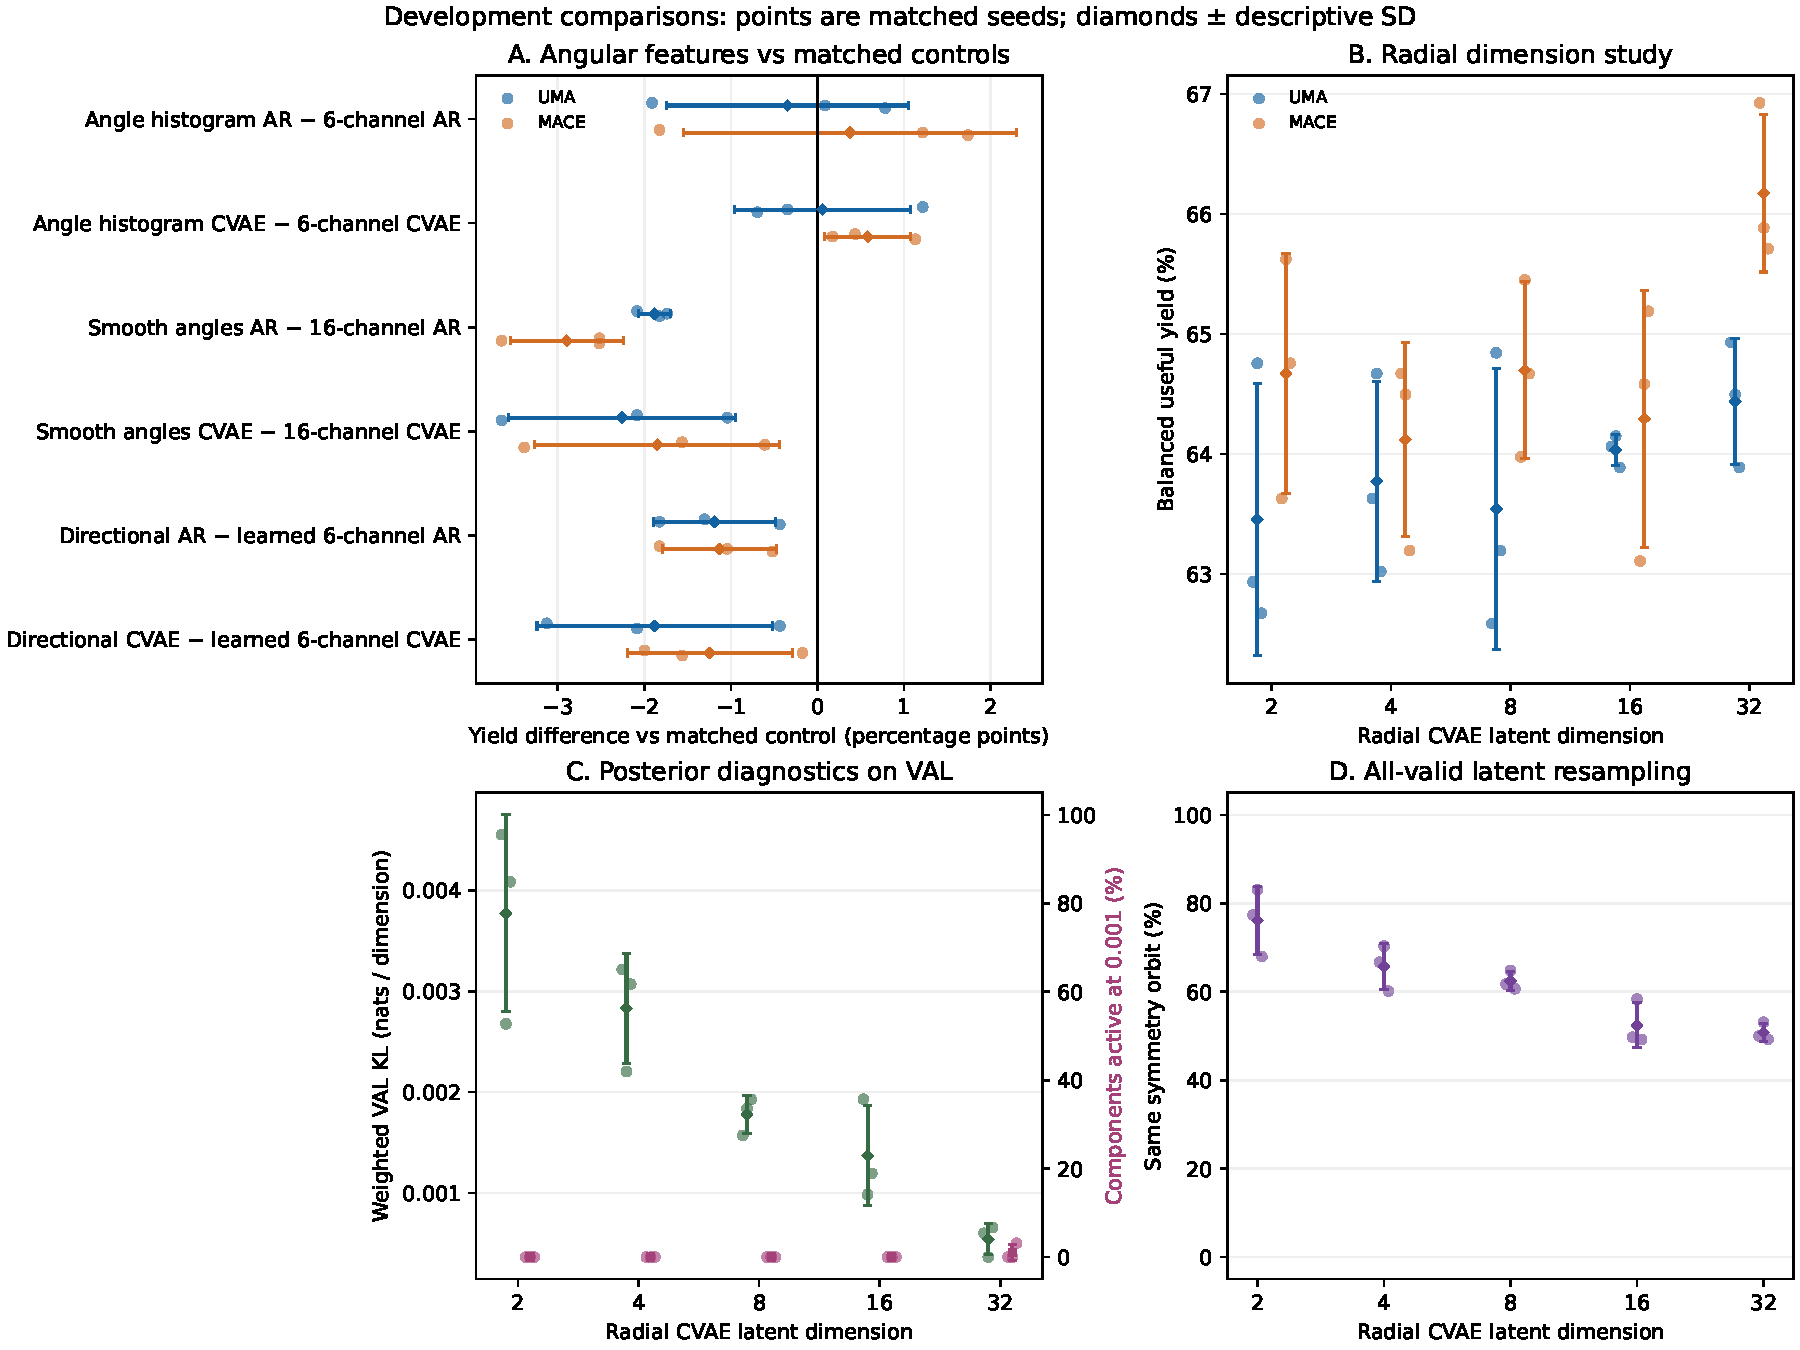
\includegraphics[width=0.94\linewidth]{development_summary.pdf}
\caption{Fresh-pool development comparisons, using both MLIP teachers. Error bars describe between-fit variation. See the associated CSV and receipt for definitions and exact controls.}
\end{figure}

\section{Angular and latent results}
On UMA, the $D=4$ radial CVAE achieves $63.77\pm0.83$\% balanced yield, radial AR $64.09\pm2.04$\%, fixed mutation $59.23\pm1.18$\%, and unconditional uniform sampling $33.33$\%. The last sampler is not conditioned on the requested bin, and the bin-averaged design partly explains its one-third result. The matched angle-histogram CVAE changes yield by $+0.06\pm1.02$ percentage points relative to its radial-width control; the smooth and directional variants change it by $-2.26\pm1.31$ and $-1.88\pm1.36$ points, respectively. The present angular features therefore do not establish an improvement; they also do not rule out better descriptors or other conditions.

Across radial $D=2$ through 32, mean UMA yields fall in a narrow 63.45--64.44\% range, but three fits at each size do not prove convergence. A low posterior KL divergence or small variance of the encoder mean $\boldsymbol\mu(\mathbf{x},c)$ suggests little information about individual training masks is encoded in the approximate posterior relative to the prior. This does not imply that the decoder ignores $\mathbf{z}$: with the same other random draws, replacing $\mathbf{z}$ changes the generated orbit in about 34\% of valid paired radial $D=4$ draws and about 52\% for smooth-angle $D=32$. This diagnostic includes protected identities, uses no energy, and is conditional on valid pairs. It establishes sensitivity to an input, not useful disentanglement, energy control, or posterior information. The 69 positive-dimensional checkpoint/sidecar pairs were separately verified to agree.

\begin{figure}[htbp]
\centering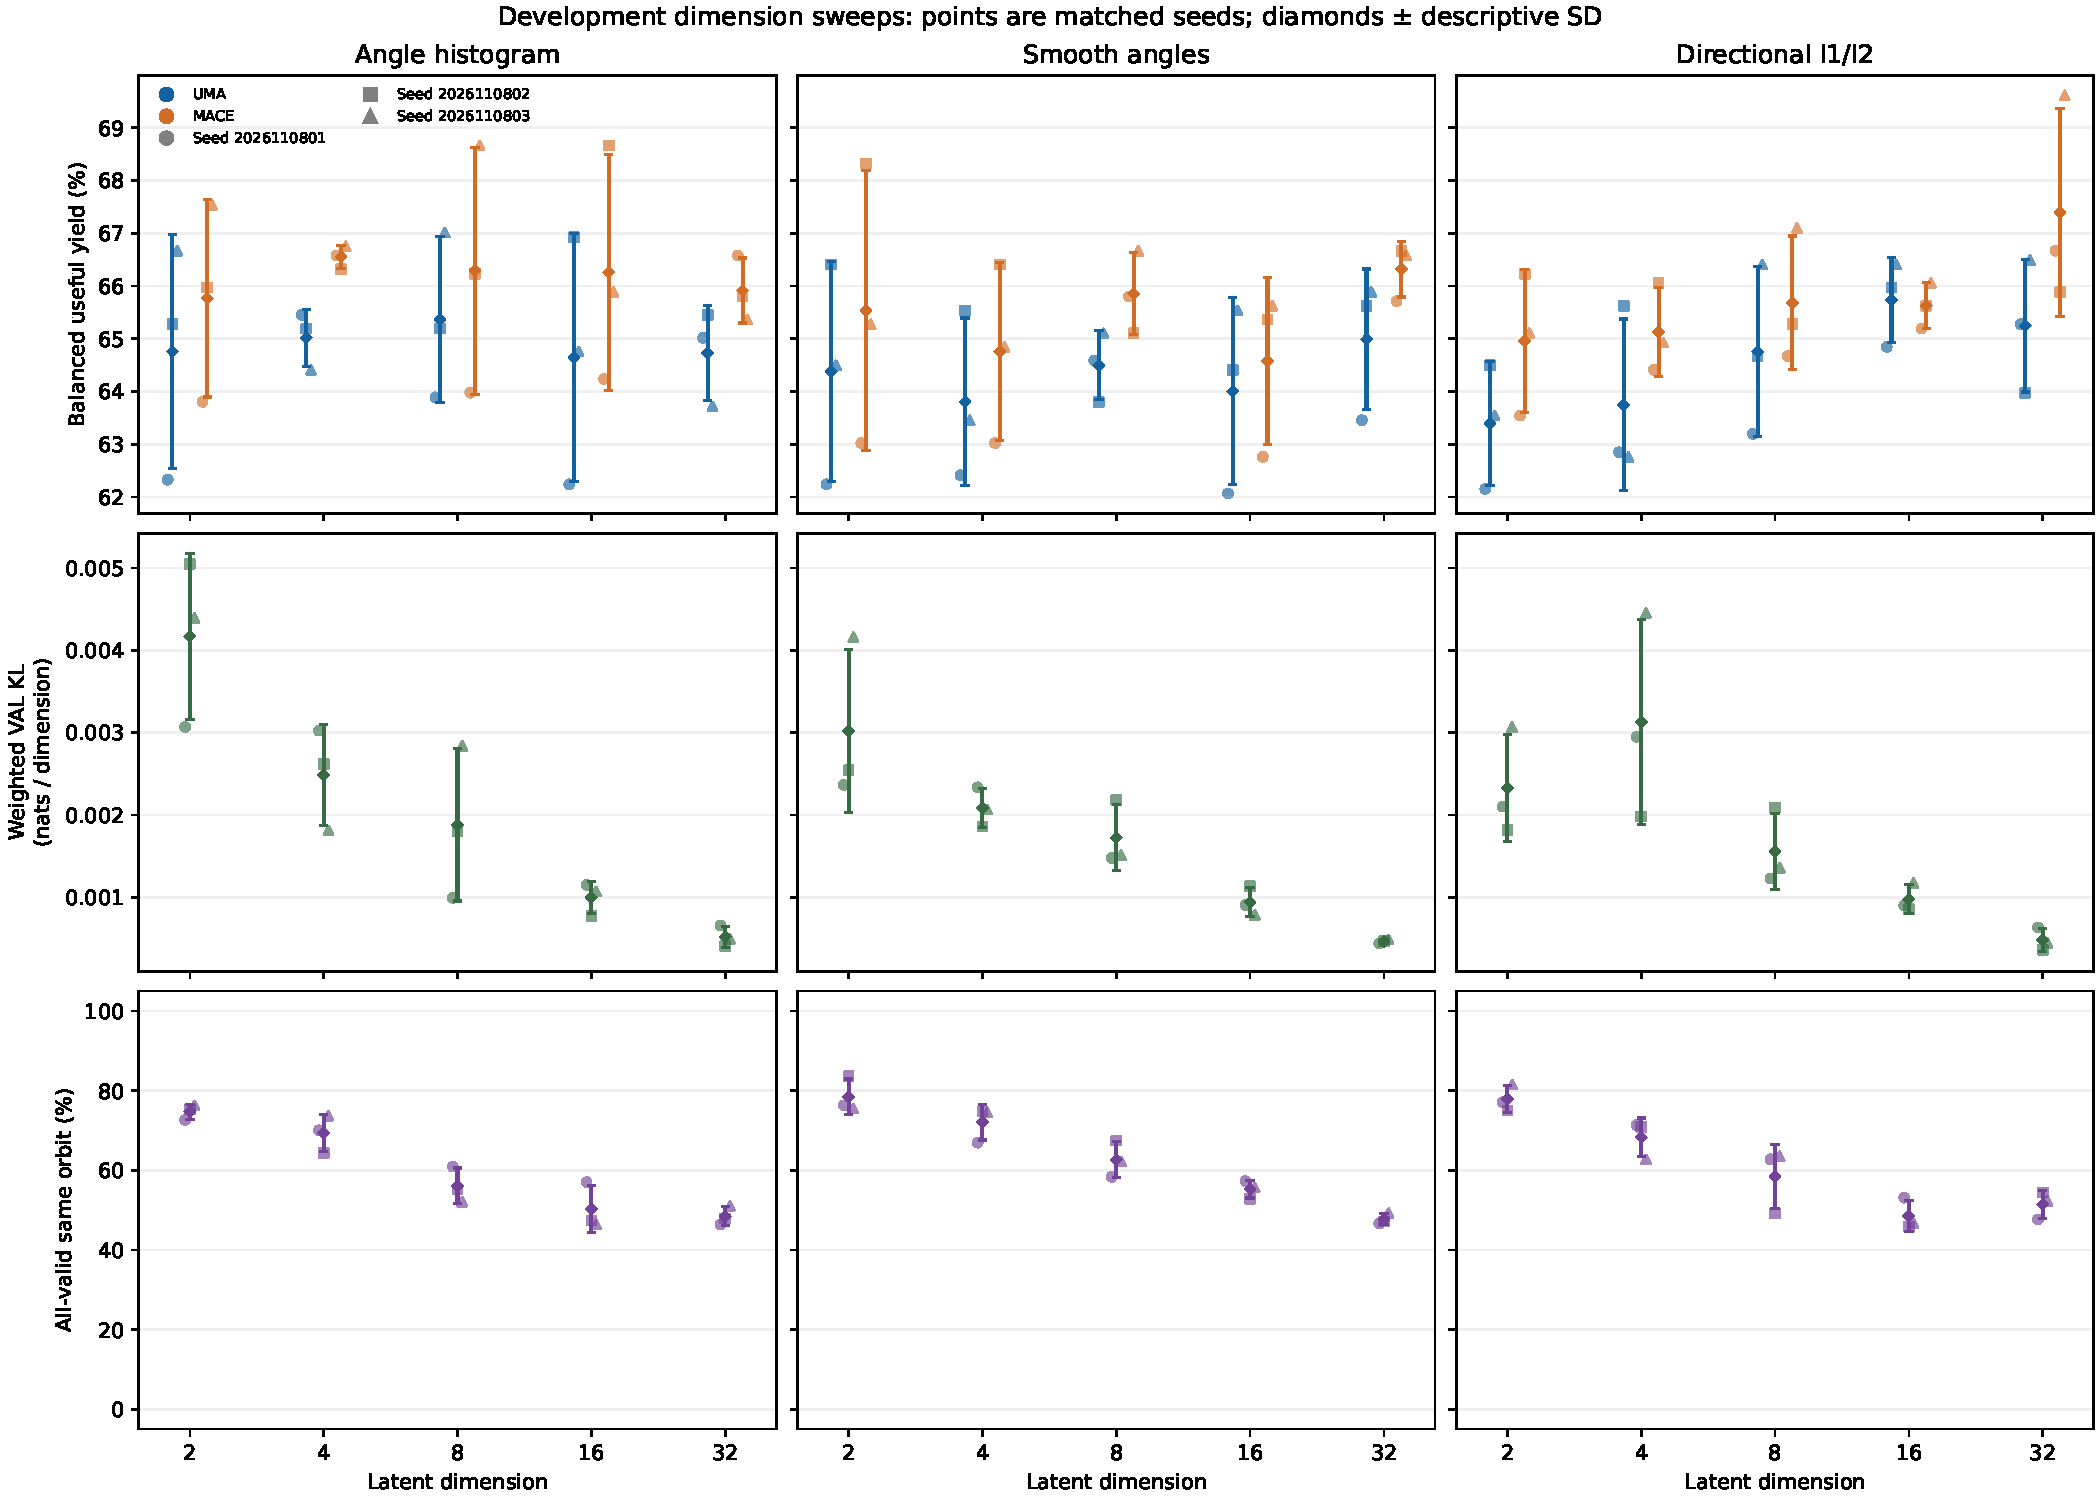
\includegraphics[width=0.95\linewidth]{angular_dimension_sweeps.pdf}
\caption{Latent-dimension sweep and diagnostic interventions. Values are development-pool results, not independently validated generalization or convergence guarantees.}
\end{figure}

On the same finite set of development candidates, UMA--MACE within-composition rank correlations were 0.972--0.986 (Spearman) and the overlap of their empirical lowest fifths was 85--89\%. These teachers often agree, but do not produce identical ranks; agreement between MLIPs does not establish agreement with DFT.

\section{Iterative acquisition: design and first round}
Wakamiya and Ishikawa \cite{wakamiya} generated catalyst candidates with a CVAE, evaluated their properties with a neural-network potential, added new samples and retrained across iterations. Our test adapts that idea to vacancy configurations; unlike their two-property labels and changing percentile labels, we retain fixed energy-bin boundaries and explicitly compare acquisition to continued training without new labels.

We selected a $D=4$ redundant-radial CVAE by a predeclared development-pool rule; its small advantage over the next family does not establish superiority. Each acquisition proposes 256 masks per composition and can add either 16 or 128 new unique UMA-scored structures per composition to TRAIN. Candidate counts and scoring caps are matched; mutation uses a fixed pre-existing TRAIN seed bank and matched random edit streams within its peer arms. CVAE proposals have no parent edit, so they do not have identical edit budgets to mutation. Existing VAL and TEST roles are preserved. Warm starts use model weights, a new optimizer and random stream, and 1,000 updates; the KL schedule restarts and does not reach its nominal final value within those updates. Primary results use the final update, with validation-selected checkpoints as a sensitivity analysis.

For first-round 128-per-composition CVAE acquisition with unit weights, the paired change relative to the no-new-data continuation is $+0.03\pm0.10$ percentage points in balanced UMA yield and $+0.75\pm1.66$ points using MACE on the same candidates. The fixed historical low-tail metric changes by $+1.22\pm1.73$ and $+1.56\pm2.64$ points, respectively. The strongest justified interpretation is that this test found little balanced-yield benefit; the small sample does not tightly determine every low-tail effect. A 20\% per-cell added-data weighting sensitivity concentrated the effective training weight (weight-based effective sample sizes roughly 1,600--1,800 versus roughly 31,000 with unit weights), rather than supplying that many statistically independent examples. For the same first-round candidate labels, 20\% weighting minus unit weighting changed balanced UMA yield by $-0.14\pm0.22$ points.

\section{A second acquisition round}
The second round evaluates untouched, first-round, and second-round models on one fresh proposal history. In addition to the general no-new-data continuation, each acquisition lineage has its own control: the same first-round checkpoint and data receive another 1,000 updates without a second acquired batch. Thus the paired difference measures the effect of the acquisition-and-retraining policy conditional on that first-round lineage. The new rows also alter class weights and minibatches, so this comparison does not isolate a fixed sequence of training examples. Novelty histories differ between rounds, so their absolute yields cannot be compared directly.

Under UMA, adding 128 CVAE-proposed labels per composition changes balanced yield by $-0.69\pm2.30$ percentage points relative to its same-lineage control; the individual paired differences are $-2.69$, $-1.22$, and $+1.82$ points. The fixed-low-tail change is $+0.09\pm2.87$ points. The corresponding mutation-acquisition change is $-0.06\pm1.20$ points in balanced yield and $+1.39\pm1.48$ points in fixed-tail yield. These are descriptive paired seed deviations, and neither policy shows a reliable general improvement from the second batch. As a separate comparison within this same second-round assessment, two successive no-new-data continuations differ from the untouched checkpoint by $+2.31\pm0.51$ points in balanced UMA yield. Further training without new labels can therefore change measured yield; the comparison remains conditional on this teacher and finite assessment pool. Improvement over an untouched model alone would not isolate acquisition benefit.

The same second-round CVAE comparison measured by MACE gives $-0.29\pm2.51$ points in balanced yield and $-0.69\pm3.36$ points in the fixed-low-tail metric. Mutation acquisition gives $-0.29\pm1.89$ and $+0.52\pm2.07$ points, respectively. Neither teacher shows a compelling balanced-yield benefit in this comparison; their mean CVAE fixed-tail changes even have opposite signs, and observed variation is large relative to the mean effects. Different second-round CVAE weight policies proposed partly different candidates; their contrast is an adaptive-policy comparison, not a clean weighting-only ablation.

\begin{figure}[htbp]
\centering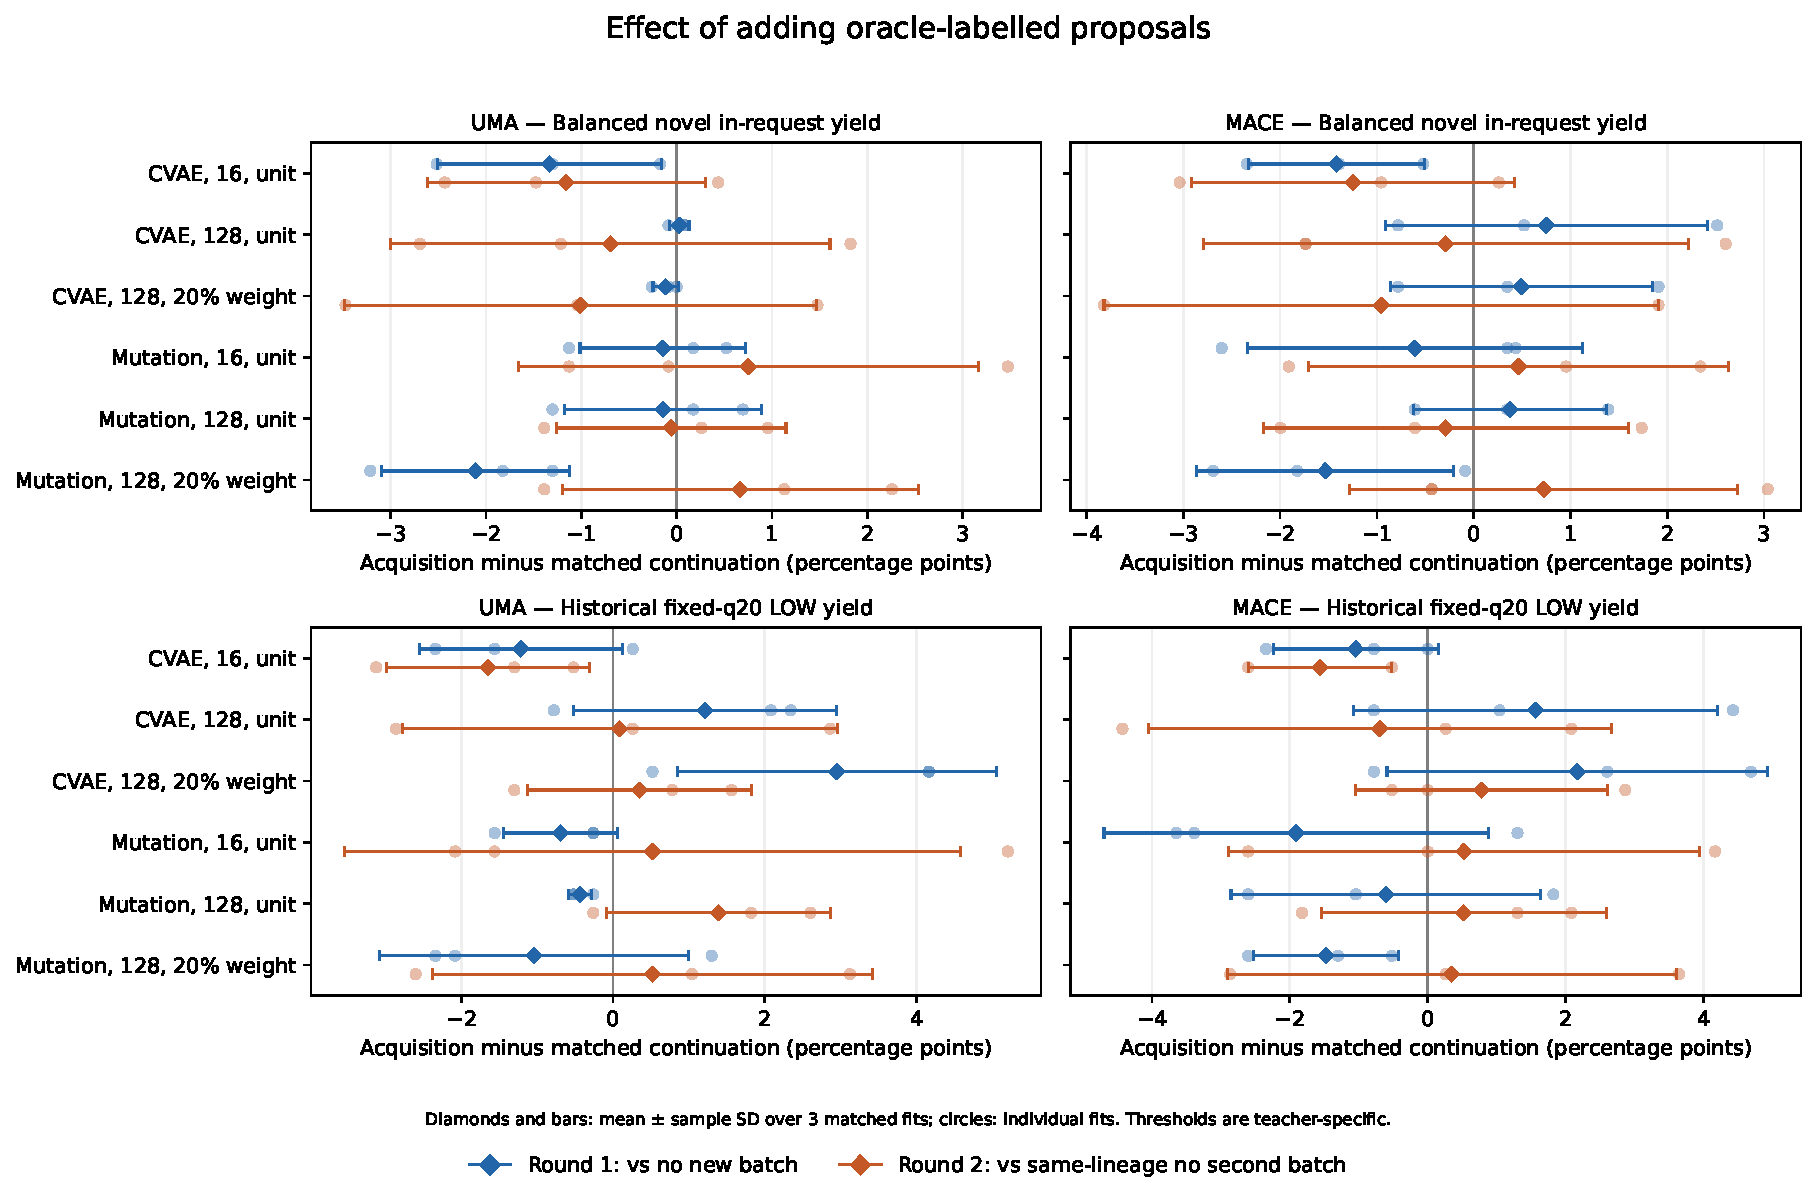
\includegraphics[width=0.96\linewidth]{iteration_paired_effects.pdf}
\caption{Each point is a seed-paired change relative to the appropriate no-new-batch continuation; diamonds and bars show the mean and sample standard deviation. Round 1 and round 2 use different assessment histories. Fixed-tail thresholds are teacher-specific and do not identify the true global lowest fifth.}
\end{figure}

\section{Interpretation and further validation}
The results favor treating the current radial AR/CVAE models and mutation as practical baselines before committing to a more complex angular architecture. The next discriminating tests are more independent fits, controlled changes to feature neighborhoods or latent objectives, and physically independent evaluation: relaxation and DFT calculations on a predeclared representative set, with a check of ranking and force errors. Generalization to different cells, other compositions or phases, and physically relaxed structures remains untested. More data or repeated self-training may amplify a teacher's own errors; MACE agreement alone does not resolve that issue.

The saved experimental record includes negative results, failed or timed-out technical runs, prospective selection rules, raw proposals, scoring receipts, and data-boundary disclosures. One helper displayed two historical protected FINAL result rows after the plans had been frozen; those numbers were not used in the selection. An earlier training implementation materialized TEST energies and saved a coarse TEST bin-support aggregate, but did not use TEST labels for gradients, loss, or checkpoint selection. The second-round implementation restricts label processing and support statistics to TRAIN/VAL; the compressed input array is still loaded. Earlier H0 TRAIN overlaps with historical protected identities were preserved as inherited; newly scored acquisition and assessment proposals exclude those protected identities. The fast final audit uses a tested post-freeze caching optimization, explicitly recorded in its receipt; the original unoptimized comparison timed out. These limitations prevent describing the run as completely blind to all historical protected information.

\begin{thebibliography}{9}
\bibitem{wakamiya} T. Wakamiya and A. Ishikawa, ``Artificial catalyst generation for the oxygen reduction reaction using conditional variational autoencoder and atomistic calculations,'' \emph{npj Computational Materials}, 12, 206 (2026). \url{https://doi.org/10.1038/s41524-026-02075-0}.
\end{thebibliography}
\end{document}
